
\subsection{Análisis de etapa en seguidor por emisor, $Q_{11}$}

\subsubsection{Análisis de la ganancia de tensión}

Dado que este circuito no cumple la condición, $r_{o} \gg R_{E}$ no se puede usar la expresión aproximada $A_{v} \approx \frac{gm \cdot R_{E}}{1 + gm \cdot R_{E}}$, con lo que tenemos:

\begin{equation}
A_{v_{Q_{11}}} = \frac{1}{1 + \frac{r_{\pi_{11}}}{  \left(  \beta_{11} + 1 \right) \cdot \left(  R_{i_{B_{Q_{7}}}} \parallelresistors r_{o_{11}}  \right)  } }
\end{equation}

\begin{equation*}
A_{v_{Q_{11}}} = \frac{1}{1 + \frac{10.1 \si[per-mode=symbol]{\kilo\ohm}}{  \left(  324 + 1 \right) \cdot \left(  1.47 \si[per-mode=symbol]{\mega\ohm} \parallelresistors 50.9 \si[per-mode=symbol]{\kilo\ohm}  \right)  } } = 0.999
\end{equation*}


\subsubsection{Análisis de la resistencia de entrada}

Para calcular la  resistencia de entrada, vemos que no se cumple la condición $r_{o} \gg R_{E}$, con lo que la expresión aproximada, $ R_{i_{B_{Q_{3}}}} \approx r_{\pi_{3}} + \beta_{3} \cdot R_{E}$ no se puede usar.\\ \\

Tenemos entonces:

\begin{equation}
R_{i_{seguidor_{Q_{11}}}} = R_{i_{B_{Q_{11}}}} = r_{\pi_{11}} + \left( \beta_{11} + 1 \right) \cdot  \left(  R_{i_{seguidor_{Q_{7}}}} \parallelresistors R_{20}   \right)  \cdot \frac{  r_{o_{11}} }{  r_{o_{11}} + \left(  1.47 \si[per-mode=symbol]{\mega\ohm} \parallelresistors R_{20}   \right)  }
\end{equation}


\begin{equation*}
R_{i_{seguidor_{Q_{11}}}} = R_{i_{B_{Q_{11}}}} = 10.1 \si[per-mode=symbol]{\kilo\ohm} + \left( 324 + 1 \right) \cdot  \left(  R_{i_{seguidor_{Q_{7}}}} \parallelresistors 10 \si[per-mode=symbol]{\kilo\ohm}   \right)  \cdot \frac{  50.9 \si[per-mode=symbol]{\kilo\ohm} }{  50.9 \si[per-mode=symbol]{\kilo\ohm} + \left(  1.47 \si[per-mode=symbol]{\mega\ohm} \parallelresistors 10 \si[per-mode=symbol]{\kilo\ohm}   \right)  } = 2.7 \si[per-mode=symbol]{\mega\ohm}
\end{equation*}


\subsubsection{Análisis de la resistencia de salida}

\begin{equation}
R_{o_{seguidor_{Q_{11}}}} = r_{d_{11}} + \frac{   R_{11} \parallelresistors \left( R_{7} + \left[  R_{L} \parallelresistors \left( R_{S} + R_{o_{Sziklai}} \right) \right]  \right) }{\beta_{11}}  
\end{equation}


\begin{equation*}
R_{o_{seguidor_{Q_{11}}}} = 31.25 \si[per-mode=symbol]{\ohm} + \frac{   10 \si[per-mode=symbol]{\kilo\ohm} \parallelresistors \left( 10 \si[per-mode=symbol]{\kilo\ohm} + \left[  100 \si[per-mode=symbol]{\ohm} \parallelresistors \left( 0.2 \si[per-mode=symbol]{\ohm} + 114.11 \si[per-mode=symbol]{\milli\ohm} \right) \right]  \right) }{324} = 46.68 \si[per-mode=symbol]{\ohm}
\end{equation*}


\subsection{Análisis de etapa en seguidor por emisor, $Q_{7}$}



\subsubsection{Análisis de la ganancia de tensión}

\begin{equation}
A_{v_{Q_{7}}} = \frac{1}{1 + \frac{r_{\pi_{7}}}{  \left(  \beta_{7} + 1 \right) \cdot \left(  R_{23} \parallelresistors \left(  R_{7} + r_{\pi_{12}} \right) \parallelresistors r_{o_{7}}  \right)  } }
\end{equation}


\begin{equation*}
A_{v_{Q_{7}}} = \frac{1}{1 + \frac{ 14.5 \si[per-mode=symbol]{\kilo\ohm} }{  \left(  335 + 1 \right) \cdot \left(  10 \si[per-mode=symbol]{\kilo\ohm} \parallelresistors \left(  1 \si[per-mode=symbol]{\kilo\ohm} + 7.21 \si[per-mode=symbol]{\kilo\ohm} \right) \parallelresistors 117 \si[per-mode=symbol]{\kilo\ohm}  \right)  } } = 0.99
\end{equation*}


\subsubsection{Análisis de la resistencia de entrada}

\begin{equation}
R_{i_{seguidor_{Q_{7}}}} = R_{i_{B_{Q_{7}}}} = r_{\pi_{7}} + \left( \beta_{7} + 1 \right) \cdot  \left[  R_{23} \parallelresistors \left(  R_{7} + r_{\pi_{12}} \right)   \right]  \cdot \frac{  r_{o_{7}} }{  r_{o_{7}} + \left[  R_{23} \parallelresistors \left(  R_{7} + r_{\pi_{12}} \right)   \right]  }
\end{equation}


\begin{equation*}
R_{i_{seguidor_{Q_{7}}}} = R_{i_{B_{Q_{7}}}} = 14.5 \si[per-mode=symbol]{\kilo\ohm} + \left( 335 + 1 \right) \cdot  \left[  10 \si[per-mode=symbol]{\kilo\ohm} \parallelresistors \left(  1 \si[per-mode=symbol]{\kilo\ohm} + 7.21 \si[per-mode=symbol]{\kilo\ohm} \right)   \right]  \cdot \frac{  117 \si[per-mode=symbol]{\kilo\ohm} }{  117 \si[per-mode=symbol]{\kilo\ohm} + \left[  10 \si[per-mode=symbol]{\kilo\ohm} \parallelresistors \left(  1 \si[per-mode=symbol]{\kilo\ohm} + 7.21 \si[per-mode=symbol]{\kilo\ohm} \right)   \right]  } = 1.47 \si[per-mode=symbol]{\mega\ohm}
\end{equation*}

\subsubsection{Análisis de la resistencia de salida}

\begin{equation}
R_{o_{seguidor_{Q_{7}}}} = r_{d_{7}} + \frac{R_{o_{seguidor_{Q_{11}}}}}{\beta_{7}}  
\end{equation}

\begin{equation*}
R_{o_{seguidor_{Q_{7}}}} = 43.10 \si[per-mode=symbol]{\ohm} + \frac{46.68 \si[per-mode=symbol]{\ohm}}{335} = 43.24 \si[per-mode=symbol]{\ohm} 
\end{equation*}


\subsection{Transferencia del realimentador}

\begin{equation}
A_{v_{llave}} = A_{v_{Q_{11}}} \cdot A_{v_{Q_{7}}}
\end{equation}

\begin{equation*}
A_{v_{llave}} = 0.999 \times 0.99 \approx 0.99
\end{equation*}


La resistencia de salida de la llave, será la vista hacia la salida del seguidor basado en $Q_{9}$, la misma se ve en paralelo con $R_{23}$, tenemos entonces:

\begin{equation}
R_{o_{llave}} = R_{o_{seguidor_{Q_{9}}}} \parallelresistors R_{23}
\end{equation}

\begin{equation*}
R_{o_{llave}} = 43.24 \si[per-mode=symbol]{\ohm} \parallelresistors 10 \si[per-mode=symbol]{\kilo\ohm} = 43.05 \si[per-mode=symbol]{\ohm}
\end{equation*}



\subsubsection{Análisis de la ganancia de corriente de los amplificadores operacionales}


Usamos las expresiones obtenidas en la sección~\sectref{section:modelo_operacional}, adaptándolas a este caso particular.

Tenemos para la trasferencia del amplificador diferencial:

\begin{equation}
A_{v_{D_{OP}}} = \frac{R_{27}}{R_{15}}
\end{equation}

\begin{equation*}
A_{v_{D_{OP}}} = \frac{25 \si[per-mode=symbol]{\kilo\ohm}}{10 \si[per-mode=symbol]{\kilo\ohm}} = 2.5
\end{equation*}


Tenemos para la trasferencia del amplificador no inversor:

\begin{equation}
A_{v_{NI_{OP}}} = 1 + \frac{R_{18}}{R_{19}}
\end{equation}


Por lo tanto para la cascada de los dos operacionales, asumiendo la resistencia de entrada del amplificador no inversor como $\infty$, tenemos


\begin{equation}
A_{v_{OP}} = A_{v_{D_{OP}}} \cdot A_{v_{NI_{OP}}} = 2.5 \cdot \left(  1 + \frac{R_{18}}{R_{19}}   \right)
\end{equation}

Para la resistencia de entrada del diferencial con operacional tenemos:

\begin{equation}
R_{i_{D_{OP}}} = R_{12} + \left( R_{13} \parallelresistors R_{14} \right) + R_{16}
\end{equation}

\begin{equation*}
R_{i_{D_{OP}}} = 10 \si[per-mode=symbol]{\kilo\ohm} + \left( 10 \si[per-mode=symbol]{\kilo\ohm} \parallelresistors 25 \si[per-mode=symbol]{\kilo\ohm} \right) + 10 \si[per-mode=symbol]{\kilo\ohm} = 27.14 \si[per-mode=symbol]{\kilo\ohm}
\end{equation*}



Dado que la resistencia de entrada del amplificador diferencial, $R_{i_{D_{OP}}}$, es mucho mayor a $R_{S}$ , podemos asumir que el amplificador no tomará corriente, haciendo que el factor de conversión de corriente a tensión sea justamente $R_{S}$.


\clearpage

\subsection{Cálculo de la ganancia de lazo para el lazo de corriente}

\label{section:current_loop_justification}


En la figura~\figref{fig:fig_current_loop_1}, puede verse el esquema de la fuente de alimentación como circuito realimentado, puede verse que se trata de realimentación \textbf{serie-serie}, que como es de esperarse estabiliza la ganancia de trans-conductancia.

\begin{figure}[H] %htb
\begin{center}
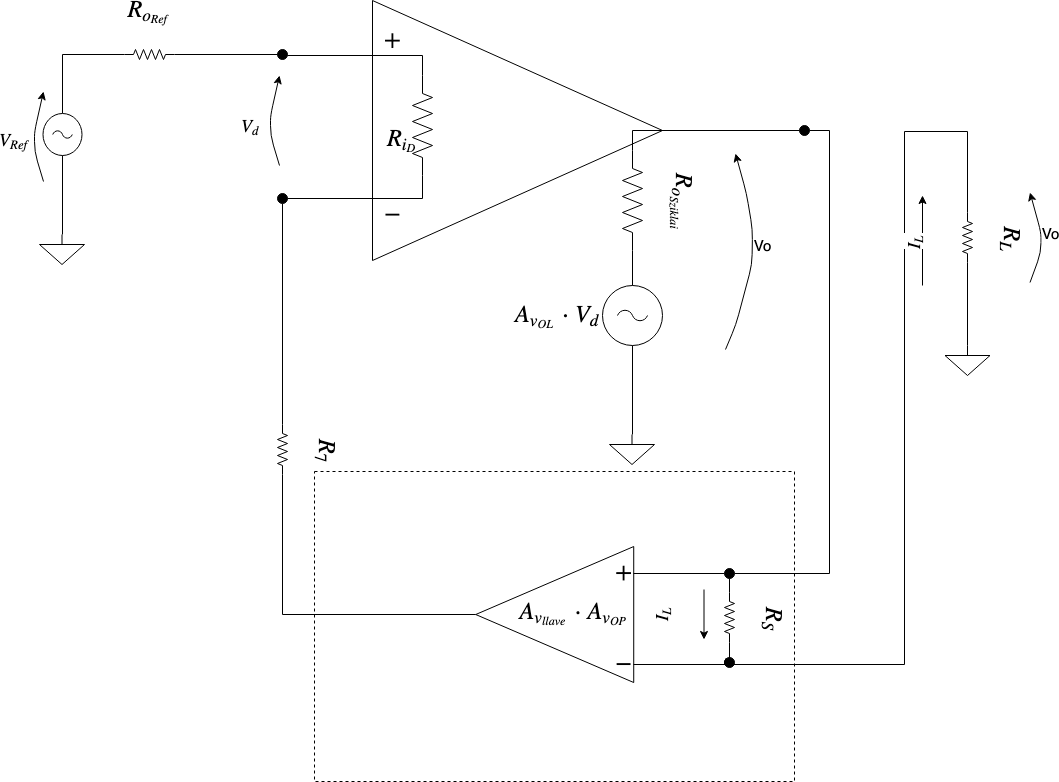
\includegraphics[width=0.9 \textwidth, angle=0]{./img/current_loop/CURRENT_LOOP_1.png}
\caption{\label{fig:fig_current_loop_1}\footnotesize{Esquema de la fuente de alimentación como circuito realimentado}}
\end{center}
\end{figure}

Aplicando parámetros \textbf{Z} al realimentador, y reordenando el circuito para llevar el realimentador a su forma ideal, se obtiene lo que se muestra en la figura~\figref{fig:fig_current_loop_2}

\vfill

\clearpage

\begin{figure}[H] %htb
\begin{center}
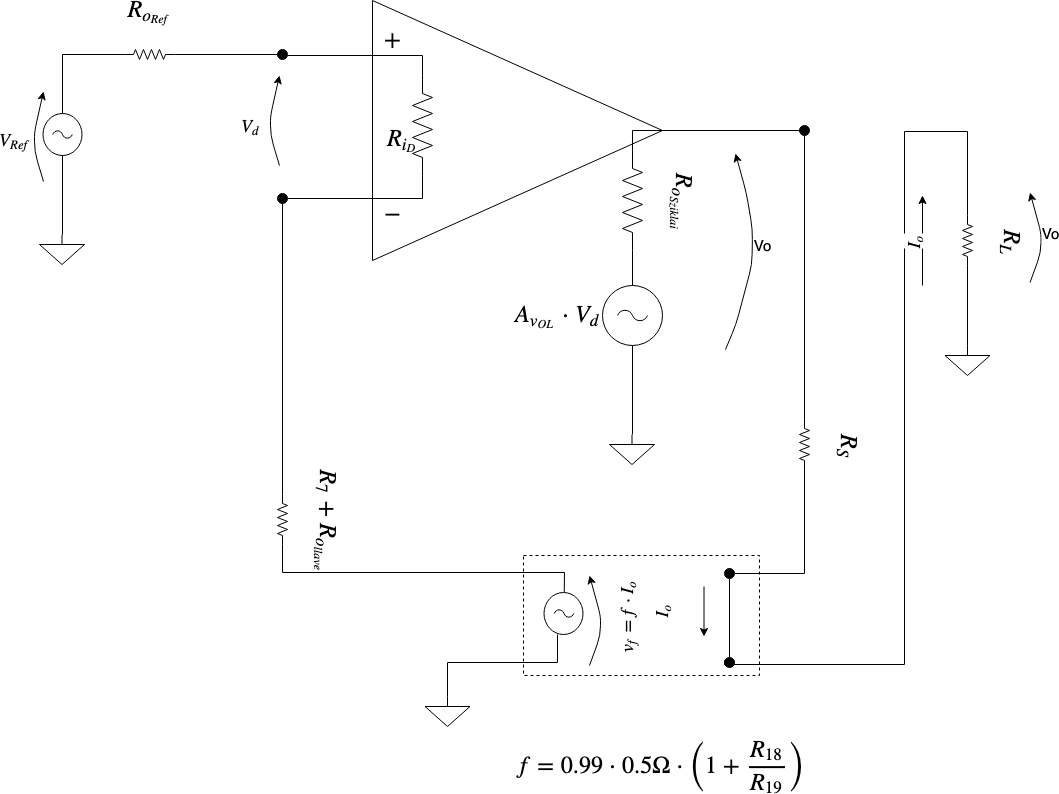
\includegraphics[width=0.9 \textwidth, angle=0]{./img/current_loop/CURRENT_LOOP_2.png}
\caption{\label{fig:fig_current_loop_2}\footnotesize{Aplicando parámetros \textbf{Z} al realimentador}}
\end{center}
\end{figure}


\begin{equation}
f = 0.99 \times 0.5 \si[per-mode=symbol]{\ohm} \times \left(  1 + \frac{R_{18}}{R_{19}} \right)
\end{equation}


\begin{equation}
a = \evalat{\frac{I_{o}}{V_{Ref}}}{f=0} = \frac{  R_{i_{D}}  }{  R_{i_{D}} + R_{o_{Ref}} + R_{7} + R_{o_{llave}}  } \cdot A{v_{OL}} \cdot \frac{1}{R_{S} + R_{o_{Sziklai}}} 
\end{equation}

\begin{equation*}
a = \frac{  15.34  \si[per-mode=symbol]{\kilo\ohm}  }{  15.34  \si[per-mode=symbol]{\kilo\ohm} + 1  \si[per-mode=symbol]{\kilo\ohm} + 1  \si[per-mode=symbol]{\kilo\ohm} + 43.05 \si[per-mode=symbol]{\ohm}  } \times 1781.51 \times \frac{1}{ 0.2 \si[per-mode=symbol]{\ohm} + 13.54 \si[per-mode=symbol]{\milli\ohm} } = 7362.21 \si{\per\ohm}
\end{equation*}





Finalmente tenemos para la ganancia de trans-conductancia a lazo cerrado:

\begin{equation}
A = \frac{a}{1 + a \cdot f}
\end{equation}

\begin{equation*}
\boxed { A = \frac{ 7362.21 \si{\per\ohm}}{1 +  7362.21 \si{\per\ohm} \times 0.99 \times 0.5 \si[per-mode=symbol]{\ohm} \times \left(  1 + \frac{R_{18}}{R_{19}} \right)} \approx 1.01 \times 2 \si{\per\ohm} \times \left( \frac{R_{19}}{R_{18} + R_{19}} \right) }
\end{equation*}

\subsection{Cálculo de la corriente de salida a lazo cerrado}


Para la corriente de salida, asumiendo una tensión de referencia de exactamente $1 \si[per-mode=symbol]{\volt}$:


\begin{equation}
\boxed { I_{o} = A \cdot V_{Ref} = 1.01 \times 2 \si[per-mode=symbol]{\ampere} \times \left( \frac{R_{19}}{R_{18} + R_{19}} \right) }
\end{equation}


\subsection{Cálculo de la resistencia de salida a lazo abierto}


La resistencia de la fuente en el nodo de salida a lazo abierto será:

\begin{equation}
R_{o_{OL}} \approx R_{o_{Sziklai}} + R_{S}
\end{equation}


\subsection{Cálculo de la resistencia de salida a lazo cerrado}


Se tendrá entonces a lazo cerrado:

\begin{equation}
R_{o} =  \left( R_{o_{Sziklai}} + R_{S} \right) \cdot \left( 1 + a \cdot f \right)
\end{equation}

\begin{equation*}
R_{o} =  \left( 13.54 \si[per-mode=symbol]{\milli\ohm} + 0.2 \si[per-mode=symbol]{\ohm} \right) \times \left( 1 + 7362.21 \si{\per\ohm} \times 0.99 \times 0.5 \si[per-mode=symbol]{\ohm} \times \left(  1 + \frac{R_{18}}{R_{19}} \right) \right) \approx 778.20 \si[per-mode=symbol]{\ohm} \times \left(  1 + \frac{R_{18}}{R_{19}} \right)
\end{equation*}

El valor de la misma depende de la realimentación como era de esperar, (también de la ganancia de lazo, esta no es estabilizada). Para el caso de $R_{18} = 0 \si[per-mode=symbol]{\ohm}$ tenemos:

\begin{equation*}
R_{o_{\left( R_{18} = 0 \si[per-mode=symbol]{\ohm} \right)}} = 1.5 \si[per-mode=symbol]{\kilo\ohm}
\end{equation*}
















